% Native editable composition from one verified, unchanged IDE capture.
\begin{figure}[htbp]
\centering
\sbox0{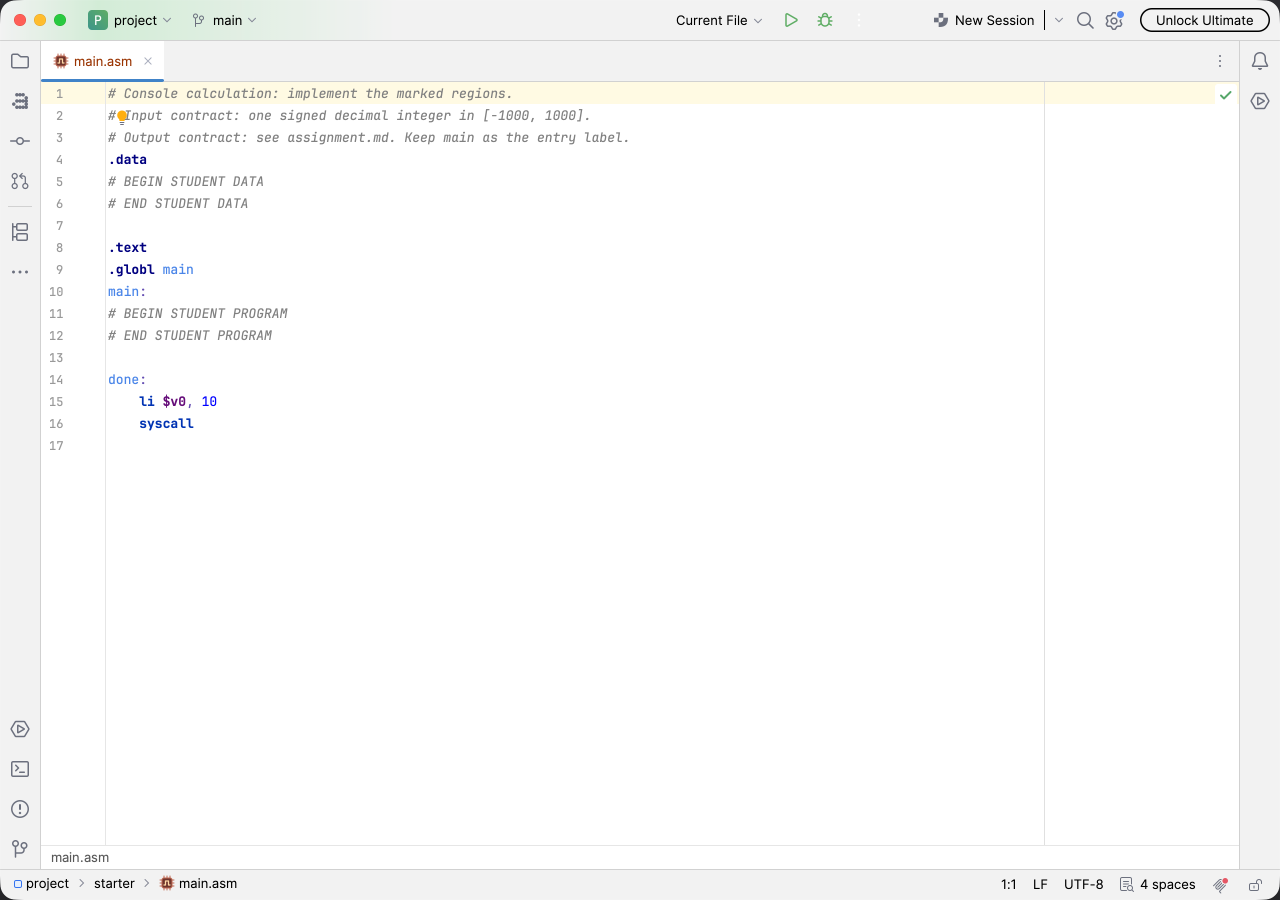
\includegraphics[artifact]{packages/001-console-calculation/captures/f01-project/raw.png}}
\edef\MARSconsoleprojectdataLeft{\the\dimexpr0.079687500\wd0\relax}
\edef\MARSconsoleprojectdataBottom{\the\dimexpr0.757777778\ht0\relax}
\edef\MARSconsoleprojectdataRight{\the\dimexpr0.685937500\wd0\relax}
\edef\MARSconsoleprojectdataTop{\the\dimexpr0.160000000\ht0\relax}
\edef\MARSconsoleprojectprogramLeft{\the\dimexpr0.079687500\wd0\relax}
\edef\MARSconsoleprojectprogramBottom{\the\dimexpr0.611111111\ht0\relax}
\edef\MARSconsoleprojectprogramRight{\the\dimexpr0.685937500\wd0\relax}
\edef\MARSconsoleprojectprogramTop{\the\dimexpr0.257777778\ht0\relax}
\edef\MARSconsoleprojectexitLeft{\the\dimexpr0.079687500\wd0\relax}
\edef\MARSconsoleprojectexitBottom{\the\dimexpr0.513333333\ht0\relax}
\edef\MARSconsoleprojectexitRight{\the\dimexpr0.685937500\wd0\relax}
\edef\MARSconsoleprojectexitTop{\the\dimexpr0.405555556\ht0\relax}
\begin{tikzpicture}[alt={Three annotated details of the unchanged starter in IntelliJ Light. The data region contains only BEGIN and END STUDENT DATA comments. The text region declares global main and contains only BEGIN and END STUDENT PROGRAM comments after main. The supplied done label loads syscall service ten into v0 and executes syscall.}]
\node[anchor=north west,inner sep=0,font=\small\bfseries] (data-title) at (6mm,0) {Message declarations go in the data region};
\node[anchor=north west,inner sep=0] (data) at ([yshift=-1mm]data-title.south west) {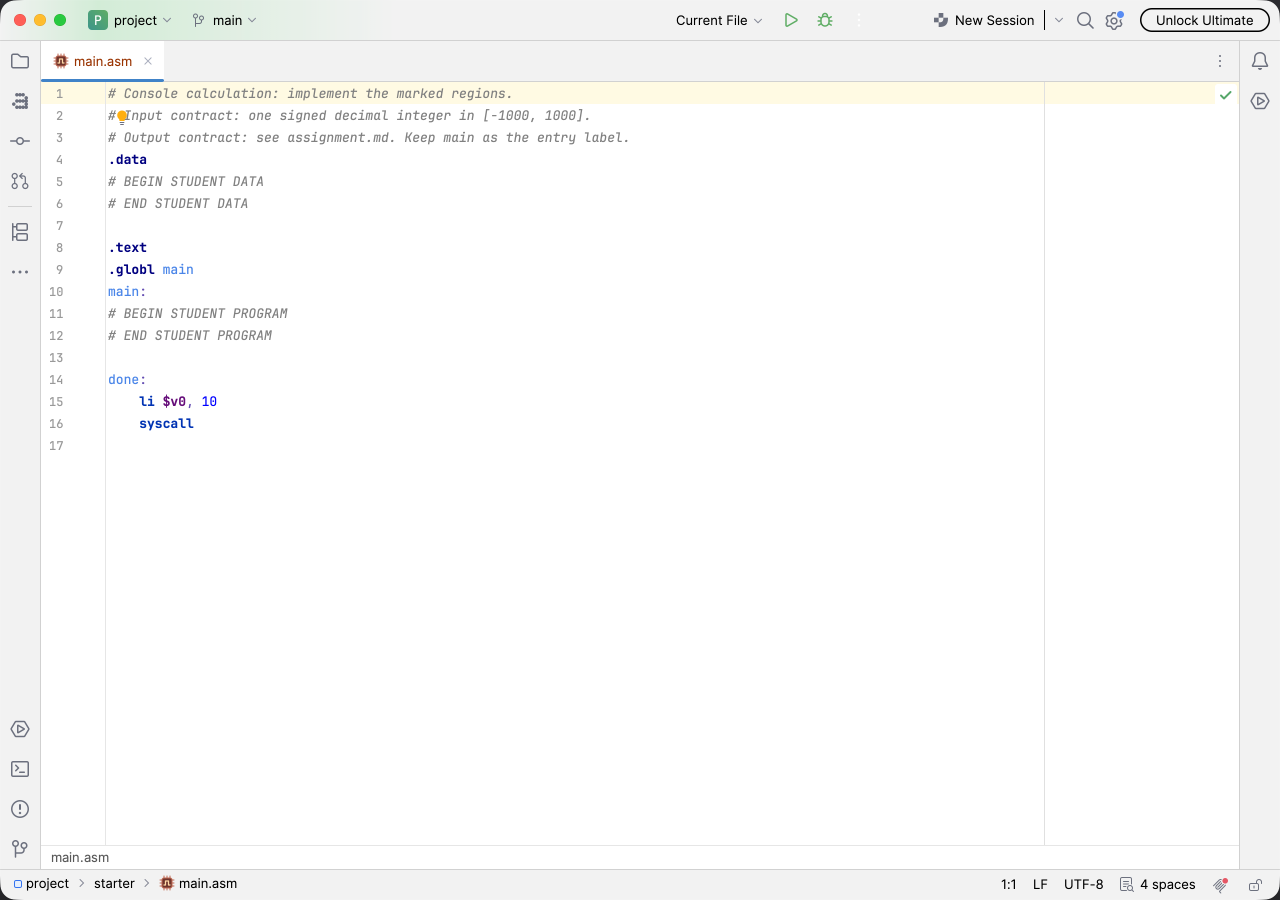
\includegraphics[width=0.66\linewidth,artifact,trim={\MARSconsoleprojectdataLeft{} \MARSconsoleprojectdataBottom{} \MARSconsoleprojectdataRight{} \MARSconsoleprojectdataTop{}},clip]{packages/001-console-calculation/captures/f01-project/raw.png}};
\begin{scope}[shift={(data.south west)},x={($(data.south east)-(data.south west)$)},y={($(data.north west)-(data.south west)$)}]
\draw[black,line width=0.7pt] (0.020000000,0.054054054) rectangle (0.540000000,0.648648649);
\node[draw=black,fill=white,circle,inner sep=1.5pt,font=\footnotesize] at ($(0.020000000,0.648648649)+(-3mm,0)$) {1};
\end{scope}
\node[anchor=north west,inner sep=0,font=\small\bfseries] (program-title) at ([yshift=-2mm]data.south west) {Instructions go after the entry label};
\node[anchor=north west,inner sep=0] (program) at ([yshift=-1mm]program-title.south west) {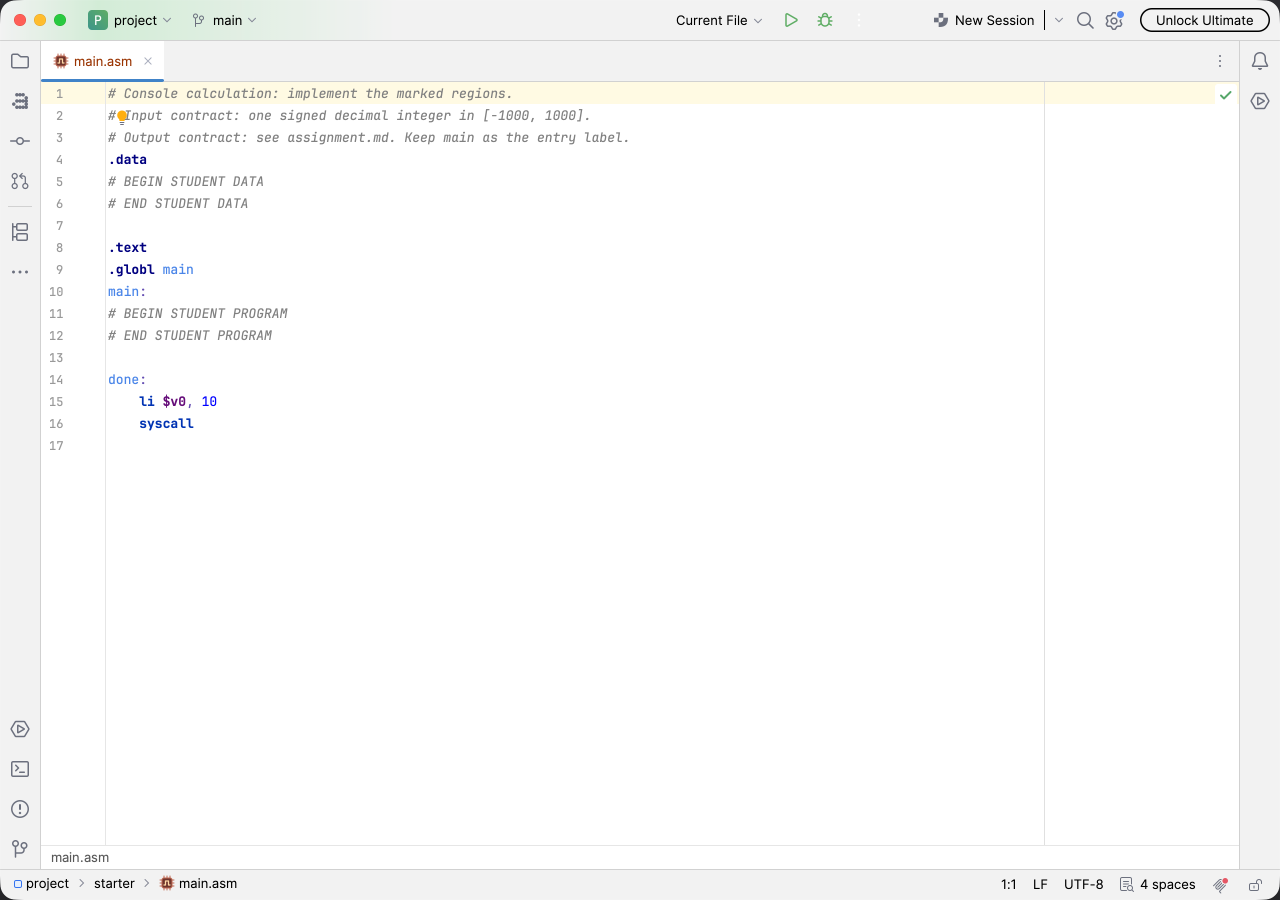
\includegraphics[width=0.66\linewidth,artifact,trim={\MARSconsoleprojectprogramLeft{} \MARSconsoleprojectprogramBottom{} \MARSconsoleprojectprogramRight{} \MARSconsoleprojectprogramTop{}},clip]{packages/001-console-calculation/captures/f01-project/raw.png}};
\begin{scope}[shift={(program.south west)},x={($(program.south east)-(program.south west)$)},y={($(program.north west)-(program.south west)$)}]
\draw[black,line width=0.7pt] (0.020000000,0.033898305) rectangle (0.616666667,0.406779661);
\node[draw=black,fill=white,circle,inner sep=1.5pt,font=\footnotesize] at ($(0.020000000,0.406779661)+(-3mm,0)$) {2};
\end{scope}
\node[anchor=north west,inner sep=0,font=\small\bfseries] (exit-title) at ([yshift=-2mm]program.south west) {The supplied exit ends the starter};
\node[anchor=north west,inner sep=0] (exit) at ([yshift=-1mm]exit-title.south west) {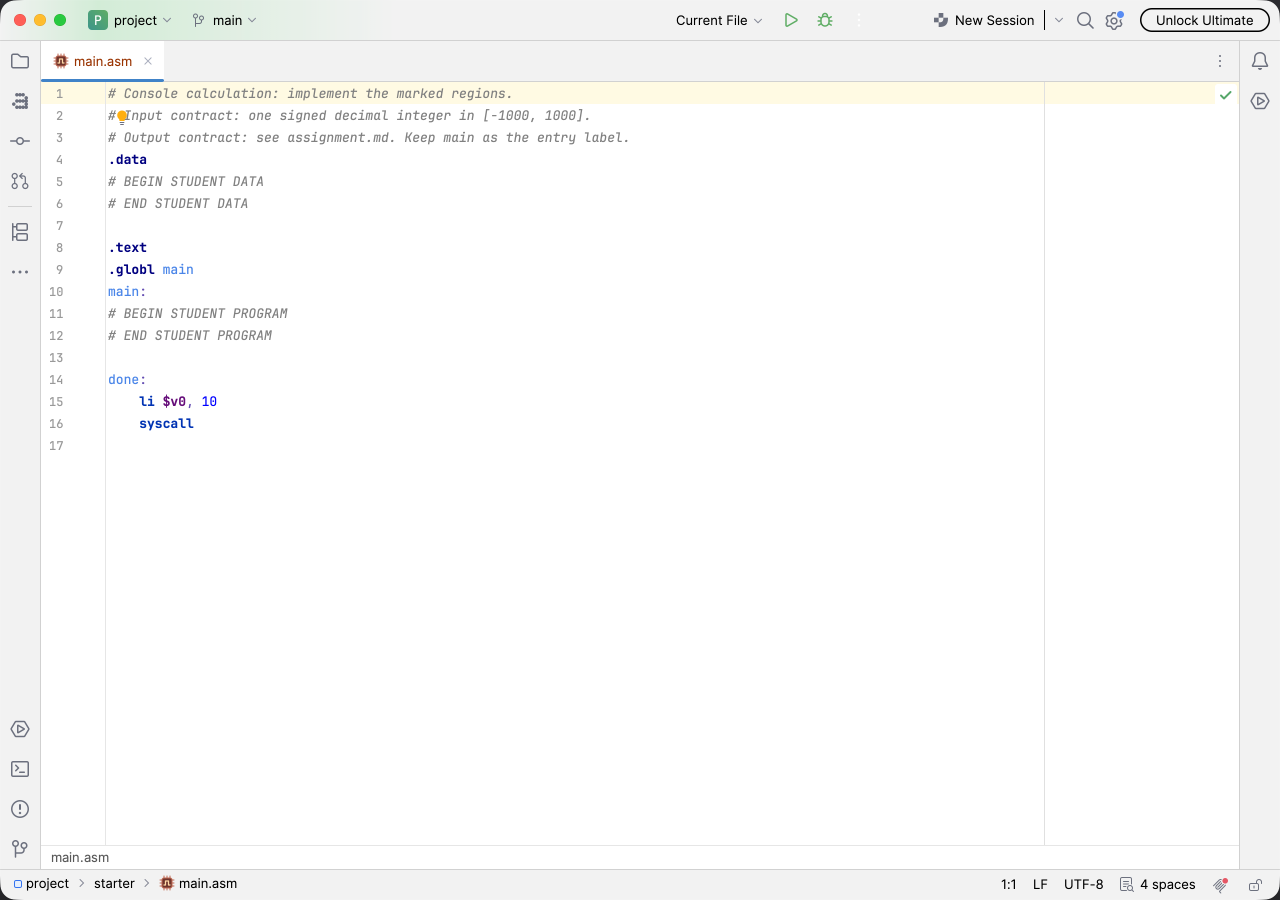
\includegraphics[width=0.66\linewidth,artifact,trim={\MARSconsoleprojectexitLeft{} \MARSconsoleprojectexitBottom{} \MARSconsoleprojectexitRight{} \MARSconsoleprojectexitTop{}},clip]{packages/001-console-calculation/captures/f01-project/raw.png}};
\begin{scope}[shift={(exit.south west)},x={($(exit.south east)-(exit.south west)$)},y={($(exit.north west)-(exit.south west)$)}]
\draw[black,line width=0.7pt] (0.020000000,0.054794521) rectangle (0.383333333,0.958904110);
\node[draw=black,fill=white,circle,inner sep=1.5pt,font=\footnotesize] at ($(0.020000000,0.958904110)+(-3mm,0)$) {3};
\end{scope}
\end{tikzpicture}
\par\smallskip
\begin{minipage}{\linewidth}
\small
\begin{enumerate}
\item \texttt{.data} selects the data region. Add the message declarations between these comments; the comments themselves do not allocate bytes.
\item \texttt{.text} selects instructions, and \texttt{main:} names the entry used by this program. Insert the program between its two marker comments. The supplied directives and entry label stay in place.
\item The exit sequence loads service ten into \texttt{\$v0} and invokes it with \texttt{syscall}. With the student region still empty, execution reaches this sequence and terminates without printing.
\end{enumerate}
\end{minipage}
\caption{The starter before any student code is added. Numbered details come from one editor capture.}
\label{capture:001-console-calculation-f01-project}
\end{figure}
